This Chapter presents the design decisions taken while implementing \acrfull{wdias} and how we adopt from the systems analyzed in \cref{ch:literature}.
\cref{se:high_level_design} presents a brief discussion on how  the weather forecasting is happening and why does it need to interact with multiple data formats.
\cref{se:architectural_decisions} shows how the architectural design of the proposed solution evolved while designing and implementing \acrshort{wdias}.
\cref{se:microservice} presents microservice architectural concepts followed while developing the \acrshort{wdias}. Then the reasons behind developing \acrshort{wdias} database structure and technologies used are discussed in  \cref{se:db_struct}.
\cref{se:data_preprocess} discusses how \acrshort{wdias} enables data preprocessing and adding capabilities using extensions. Finally, \cref{se:query} includes details on how to perform timeseries search and geo-based queries on the \acrshort{wdias}.


%%%%%%%%%%%%%%%%%%%%%%%%%%%%%%%%%%%%%%%%%%%%%%%%%%%%%%%%%%%%%%%%%%%%%%%%%%%%%%%%
\section{High-level Design}
\label{se:high_level_design}

To get an overall idea of the flow of weather forecast, let us look into one of the weather forecasting flows in the \acrshort{curw} \cite{CUrWSL2017Lanka}.

\begin{enumerate}
    \item Extract \acrshort{GRIB} \acrshort{wrf} model data to the \acrshort{netCDF} format.
    \item Extract \acrshort{netCDF} data to \acrshort{csv} format for each location data, then feed to HEC-HMS hydrodynamic model and get the output as a \acrshort{csv} file.
    \item HEC-HMS's \acrshort{csv} output and precipitation as Grid files feed into the FLO2D hydrologic model and get the water level as ASCII Grid files after the simulation is complete.
    \item Upload above ASCII files to a geographic information system after convert to a compatible format, then use for the loss estimation.
\end{enumerate}
    
In the above weather forecasting steps, we can see that the weather data need to convert to different formats while feeding from one model or step to another. After the models run successfully, the resulting output data may not be accurate or biased based on different factors. In such situations, we need to correct predicted weather data by comparing them with accurate real-time weather data. We are required to collect real-time data from automated weather stations and accumulated weather data over a given period by automatic water level stations.

Most weather data collecting devices use own data formats and different standard protocols to transmit the data. Then we need to validate the data and modify the data to remove errors. Also, these data need to convert into model compatible data format before feeding into models. The models output data in different formats and need to store those bulk data efficiently, and the system should be flexible enough to upgrade to support new data formats easily. Essentially, the system should share the real data, forecasted data, and other created data with relevant parties based on authorization.


%%%%%%%%%%%%%%%%%%%%%%%%%%%%%%%%%%%%%%%%%%%%%%%%%%%%%%%%%%%%%%%%%
% \subsection{Modules of a Weather Data System}
% \label{subse:modules_weather_data_integration_sys}

\cref{fi:wdia_components} shows the basic functions of a weather data integration and assimilation system consisting of the following modules: 

\begin{figure}[htbp]
\centerline{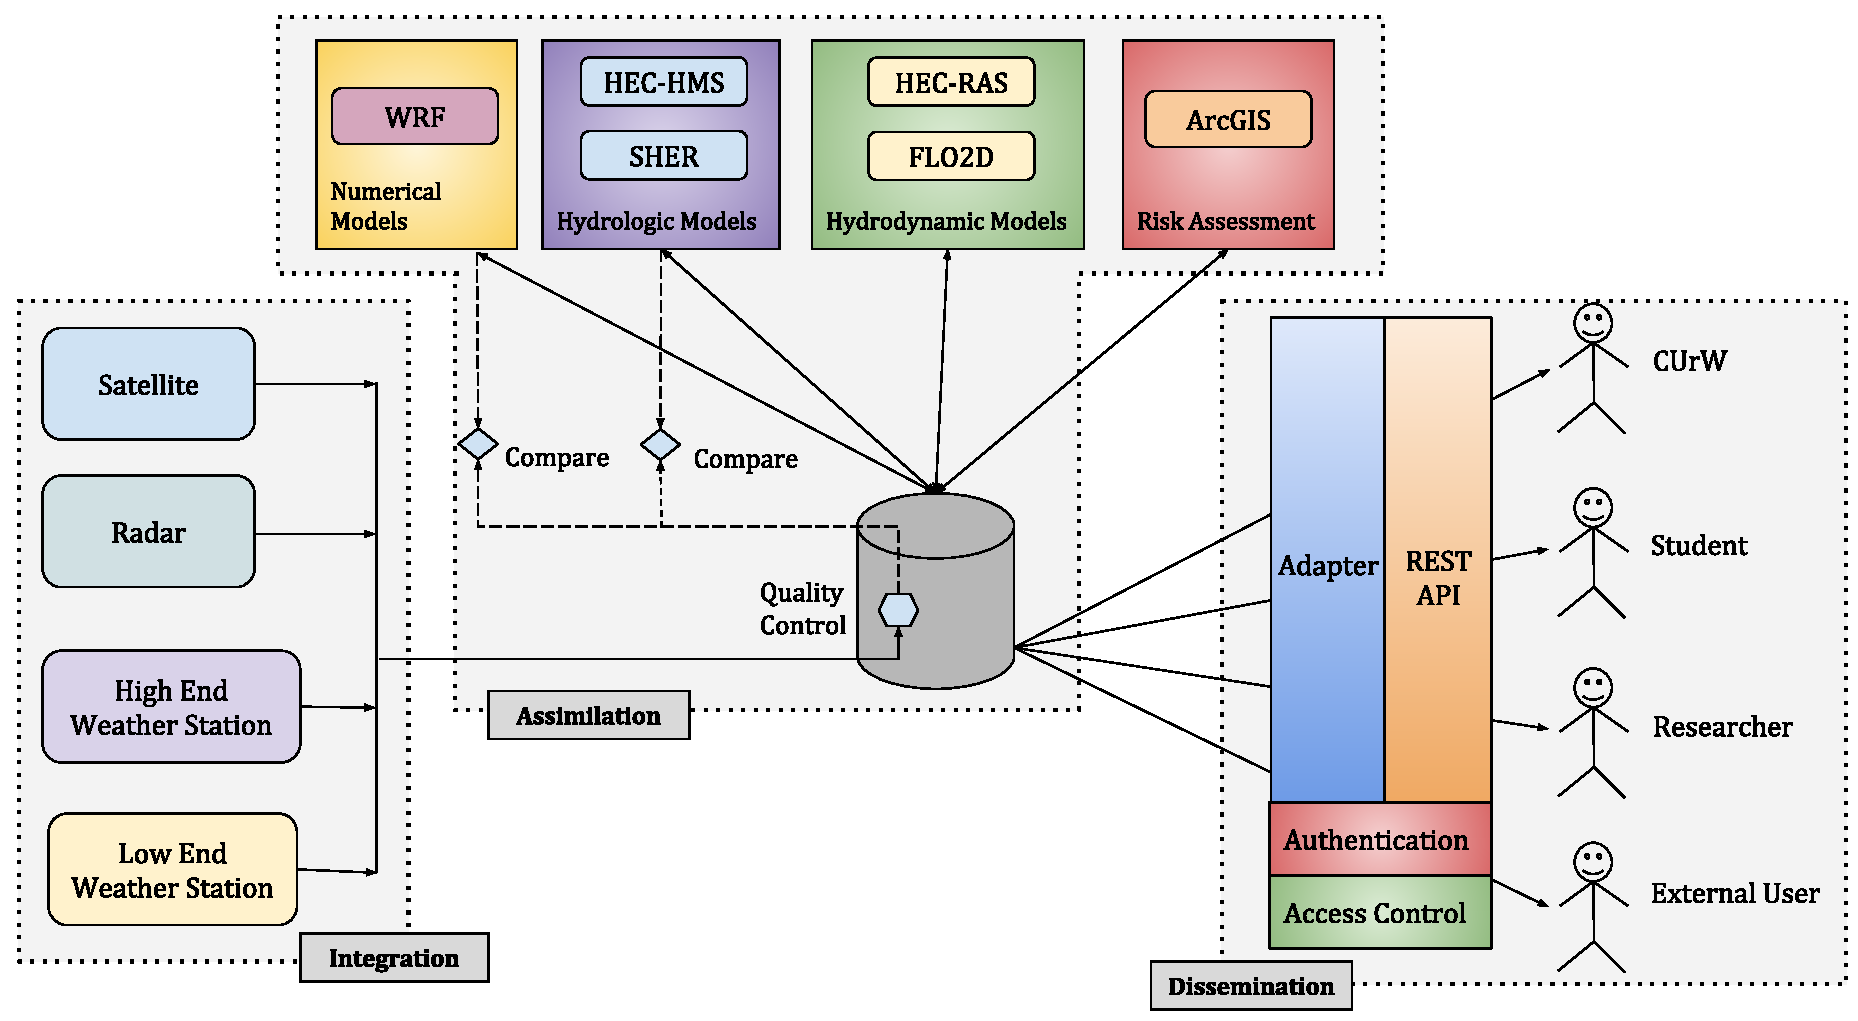
\includegraphics[width=1\textwidth]{method/misc/weather_data_system_components.pdf}}
\caption{Modules of a weather data system.}
\label{fi:wdia_components}
\end{figure}

\subsubsection{Integration }
The system should be capable of integrating data from different sources such as satellite data, high end, and low-end weather station. And the system should be able to handle multidimensional spatial and temporal weather data efficiently and optimally.
\subsubsection{Assimilation}
Then the system should be able to fulfill weather models varying data requirements. Also, those models reproduce a large set of redundant data. Thus, the system should store the bulk data while optimizing the disk space.
\subsubsection{Dissemination}
Then different users should be able to retrieve data as they require. Also, the users should be able to easily search into the available information in the system based on timeseries metadata or based on geo-queries.
